\begin{BPMN}{PROC-04}{Carga del Resumen del Plan de Estudios}{El proceso consiste en ingresar al sistema información del Plan de Estudios que es necesaria al momento de generar los Programas de Estudio de las Unidades de Aprendizaje. Este proceso no existe en el negocio actual pero es necesario para explotar las areas de oprtunidad identificadas en el Macroproceso.}
    \PCitem{Participantes}{
    	\begin{itemize}
    		\item Jefe de Innovación Educativa
    		\item Jefe de División de Innovación Académica
    		\item Jefe de Departamento de Desarrollo e Innovación Curricular
    		\item Analista DES
    	\end{itemize}
    }
    \PCitem{Objetivo}{Subir la información escencial del Plan de Estudios para asistir en la elaboración y revisión de los Programas de Estudio de las Unidades de Aprendizaje}
    \PCitem{Interrelación con otros procesos}{
        \begin{itemize}
            \item Entrada: Recibir respuesta de aprobación del Plan de Estudios
            \item Salida: Elaborar Unidades de Aprendizaje
        \end{itemize}
    }
    \PCitem{Proveedores}{Dirección de Educación Superior}
    \PCitem{Entradas}{Aprobación del Plan de Estudios}
    \PCitem{Consumidores}{Unidad Académica}
    \PCitem{Precondiciones}{Elaboración y Aprobación del Plan de Estudios}
    \PCitem{Postcondiciones}{Elaboración de Unidades de Aprendizaje}
    \PCitem{Frecuencia}{}
    \PCitem{Tipo}{Operación}
\end{BPMN}
\newpage
\hypertarget{SP4}{\begin{figure}[htbp]
	\begin{center}
	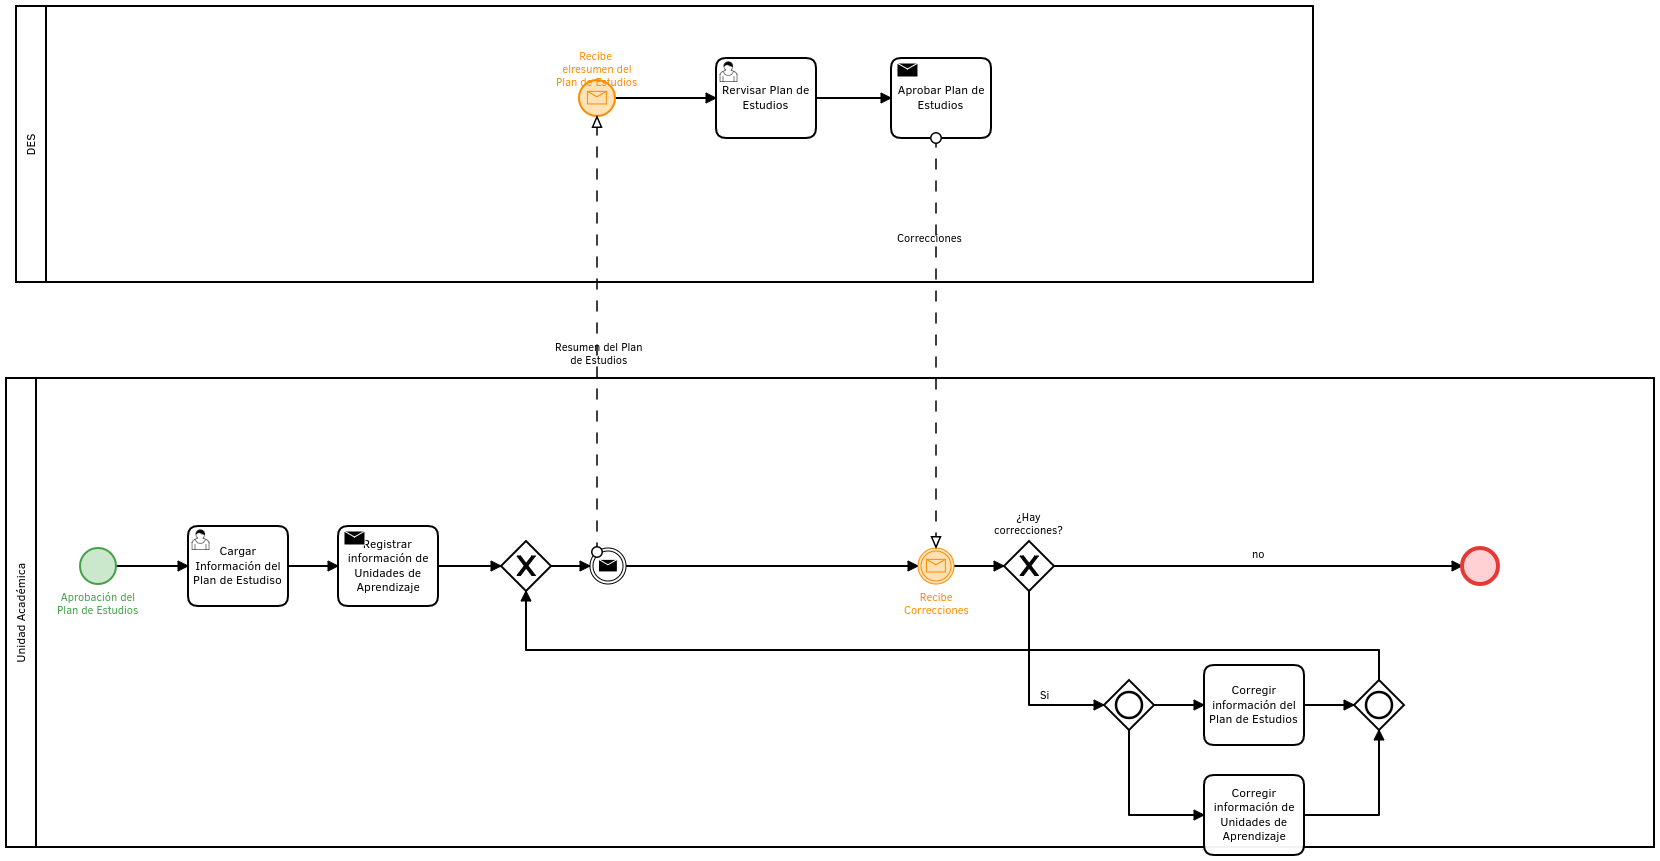
\includegraphics[width=.95\textwidth]{C1-DP/SP4/Image/SP4}
		\caption{BPMN-04 Subproceso para la carga del Plan de Estudios}
		\label{fig:BPMN-04}
	\end{center}
\end{figure}}
\begin{itemize}
    \item \textbf{Cargar Información del Plande Estudios:}\\
    El Jefe de Innovación Educativa una vez que recibe la aprobación del Plan de Estudios, ingresa al Sistema el Año, la Modalidad, Créditos TEPIC y SATCA, Total Horas/Teoría y Total Horas/Práctica del documento del Plan de Estudios.
    \item \textbf{Registrar Información de las Unidades de Aprendizaje:}\\
    El Jefe de Innovación Educativa terminado el registro del la información del Plan de Estudios, ingresa el Semestre, Nombre, Área de Formación, Horas Teoría/Semana, Horas Práctica/Semana y Creditos SATCA.
    \item \textbf{Revisar Resumen Plan de Estudios:}\\
    El Jefe de Departamento de Desarrollo e Innovación Curricular terminado el registro del Resumen del Plan de Estudios, asigna a un Analista para que verifique que la información se haya cargado de manera correcta y de ser necesario anexará las indicaciones a atender.
    \item \textbf{Aprobar Resumen Plan de Estudios:}\\
    Cuando el Analista haya finalizado su revisión, el Jefe de Departamento de Desarrollo e Innovación Curricular podra revisarlo y agregar mas anotaciones.
    \item \textbf{Corregir Información del Plande Estudios:}\\
    Si a la información del Plan de Estudios se le hizo alguna anotación ya sea en el proceso de Revisión o de Aprobación, esta tendra que ser atendida por el Jefe de Innovación Educativa. Regresa a la tarea de Revisión.
    \item \textbf{Corregir Información de las Unidades de Aprendizaje:}\\
    Si a la información de alguna de las Unidades de Aprendizaje se le hizo alguna anotación ya sea en el proceso de Revisión o de Aprobación, esta tendra que ser atendida por el Jefe de Innovación Educativa. Regresa a la tarea de Revisión.
\end{itemize}